\documentclass[ngerman,14pt,aspectratio=1610]{beamer}

% Imports
\usepackage[utf8]{inputenc}
\usepackage[T1]{fontenc}
\usepackage{babel}
\usepackage{graphicx}
\usepackage{multicol}
\usepackage{textpos} % Logo in frametitle
\usepackage{ifthen} % Für das \ifthenelse
\usepackage{totcount} % Für Counter, die in main.aux gespeichert werden
\usepackage{forest}

% Startpfad für Bilder setzen
\graphicspath{ {./images/} }

% DHBW Logos
\newcommand{\dhbwlangtrans}{
\includegraphics[width=5cm]{dhbw_lang_trans}}
\newcommand{\dhbwkurzweiss}{
\includegraphics[width=0.5\paperwidth]{dhbw}}

% Subsections zählen
\def\secname{Gliederung} % Der Titel der jeweiligen Section wird in secname gespeichert, damit innerhalb der Section der counter mit dem name erhöht werden kann
\let\oldsection\section
\renewcommand{\section}[1]{
	\oldsection{#1}
	\newtotcounter{#1}
	\def\secname{#1}
}
\let\oldsubsection\subsection
\renewcommand{\subsection}[1]{
	\oldsubsection{#1} 
	\stepcounter{\secname}
}

% Nummern bei Frametitle
\newcommand{\secpagnum}{\insertsectionnumber.\thesubsection}
\newcommand{\lastpagenum}{1}
\let\oldframetitle\frametitle
\renewcommand{\frametitle}[1]{
	\ifthenelse{\equal{\lastpagenum}{\insertslidenumber}}{
		\subsection{}
		\renewcommand{\lastpagenum}{\insertslidenumber}
	}{
		% Hier soll nichts passieren, damit bei gleichen slides der title nicht neu gesetzt wird
	}
	
	\ifthenelse{\totvalue{\secname}>1}{
	\oldframetitle{\secpagnum~#1}
	}{
	\oldframetitle{\insertsectionnumber~#1}
	}
}

% Multicol column balancing ausschalten
\raggedcolumns

% Basis-Theme
\usetheme[progressbar=frametitle, block=fill, sectionpage=none]{metropolis} % Hier kann die progressbar deaktiviert/replaziert werden
\setbeamertemplate{frame numbering}[counter]
\useoutertheme{metropolis}
\useinnertheme{metropolis}
\usefonttheme{metropolis}
\setbeamercolor{background canvas}{bg=white}

% Sections im ToC Nummerieren
\setbeamertemplate{section in toc}[sections numbered]
\setbeamertemplate{subsection in toc}[subsections numbered]

% Zeilenabstand ToC
\makeatletter
\patchcmd{\beamer@sectionintoc}
{\vfill}
{\vskip\itemsep}
{}
{}
\makeatother 

% DHBW Farben
\definecolor{dhbw_grau}{RGB}{93,104,110}
\definecolor{dhbw_rot}{RGB}{227,6,19}
\definecolor{dunkelgrau}{RGB}{41,55,67}
\definecolor{hellgrau}{RGB}{239,241,242}

% DHBW Farben einbauen
\setbeamercolor{progress bar}{fg=dhbw_rot, bg=hellgrau}
\setbeamercolor{normal text}{fg=dunkelgrau} %bg hier macht block bg
\setbeamercolor{alerted text}{fg=dhbw_rot}
\setbeamercolor{frametitle}{fg=dhbw_rot,bg=hellgrau}
\setbeamercolor{title}{fg=dhbw_rot}
\setbeamercolor{subtitle}{fg=dunkelgrau}
\setbeamercolor{section title}{fg=dhbw_rot}
\setbeamercolor{institute}{fg=dhbw_rot}

% Logo in frametitle
\addtobeamertemplate{frametitle}{}{%
	\begin{textblock*}{5cm}(\textwidth-4cm,-1.3cm)
		\dhbwlangtrans
	\end{textblock*}}

% Datum in der Fußzeile
\setbeamertemplate{frame footer}{
	\hskip 2.5em \insertdate
} 

% Endseite
\newcommand{\finalpage}[2][Vielen Dank für ihre Aufmerksamkeit!]{
\metroset{sectionpage=none}
\setbeamertemplate{frame numbering}[none]
\setbeamertemplate{frame footer}{}
\oldsection*{#1}
\begin{frame} \vspace{60pt}
	\sectionpage
	\vspace{10pt}
	\centering
	#2
\end{frame}
}

% Daten für die Titelseite
\title{Explainable-AI - Post-Hoc-Analyse - Erkennung von Hirntumoren}
%\subtitle{subtitle}
\author{Sven Sendke}
\institute[DHBW Stuttgart]{Duale Hochschule Baden-Württemberg Stuttgart}
\date{09.12.2024}	
\titlegraphic { 
	\begin{tikzpicture}[overlay,remember picture]
		\node[right=0.5cm] at (current page.155){
			\dhbwlangtrans
		};
	\end{tikzpicture}
}

\regtotcounter{section}
\regtotcounter{subsection}

\begin{document}
	
	\begin{frame}[plain,noframenumbering]
		\titlepage
	\end{frame}

	\section{Gliederung}
	
	\begin{frame}[t]{Gliederung} \vspace{20pt}
		\begin{columns}[T, onlytextwidth]
			\column{0.5\textwidth}
			\linespread{1.5}
			\tableofcontents
			\column{0.5\textwidth}
		\end{columns}
	\end{frame}
	
	\metroset{sectionpage=simple} % Erst hier definiert, damit die Gliederung keine Sectionpage hat
	\section{Einleitung}
		\begin{frame}[t]{Einleitung - Hirntumor} \vspace{5pt}
			\begin{columns}[T, onlytextwidth]
				\column{0.45\textwidth}
				\begin{itemize}
					\item \textbf{Abnormales} Wachstum von \textbf{Zellen} im Gehirn
					\item In Deutschland  erkranken \textbf{jährlich} etwa \textbf{8.000 Menschen} neu an einem Hirntumor
					\item \textbf{Zeitaufwändige} und \textbf{teure} Untersuchungsmethode
				\end{itemize}
				
				\column{0.45\textwidth}
				\includegraphics[width=\linewidth]{brain\_tumor\_1}
			\end{columns}
		\end{frame}
		
		\begin{frame}[t]{Einleitung - Herausforderungen} \vspace*{\fill}
				\begin{itemize}
					\item Einsatz von CNNs in der  \textbf{medizinischen Bildsegmentierung}
					\item Erkennung von Hirntumoren in MRT-Bildern ist schwierig aufgrund der \textbf{komplexen Gehirnstruktur}
					\item Schwierigkeit, die \textbf{Gründe} für die Antwort von CNN zu verstehen
				\end{itemize}
		\end{frame}
		
		\begin{frame}[t]{Einleitung - Forschungsfrage}
			\vspace*{\fill}
			Erstellung eines CNNs zur \textbf{Erkennung von Hirntumoren} und Anwendung von \textbf{Layer-wise Relevance Propagation} (LRP) zur Analyse der Relevanz der einzelnen Pixel für die \textbf{Entscheidungsfindung} des Netzwerks, um herauszufinden, welche \textbf{Muster} bei der Erkennung geholfen haben.
		\end{frame}
		
		\begin{frame}[t]{Einleitung - Datensatz}
			\begin{columns}[T, onlytextwidth]
				\column{0.45\textwidth}
				\vspace{50pt}
					\includegraphics[width=\linewidth]{kaggle\_1}
					\includegraphics[width=\linewidth]{kaggle\_2}
					
				\column{0.45\textwidth}
				\vspace{70pt}
					https://www.kaggle.com/
					datasets/preetviradiya/brian
					-tumor-dataset/data
			\end{columns}
		\end{frame}
		
		\begin{frame}[t]{Einleitung - Datensatz} 
			\vspace*{\fill}
			\begin{columns}[T, onlytextwidth]
				\column{0.45\textwidth}
				Probleme mit dem Datensatz:
				\begin{itemize}
					\item Doppelte Bilder
					\item Einige Bilder sind kleine Variationen
				\end{itemize}
				
				\column{0.45\textwidth}
				\begin{block}{Achtung!}
					Auf der Seite steht, es seien Röntgenbilder, aber es sind MRT / CT Bilder!!!!
				\end{block}
			\end{columns}
		\end{frame}
	
	\section{Projekt}
		\begin{frame}[t]{Projekt - GitHub Repository} \vspace{20pt}
			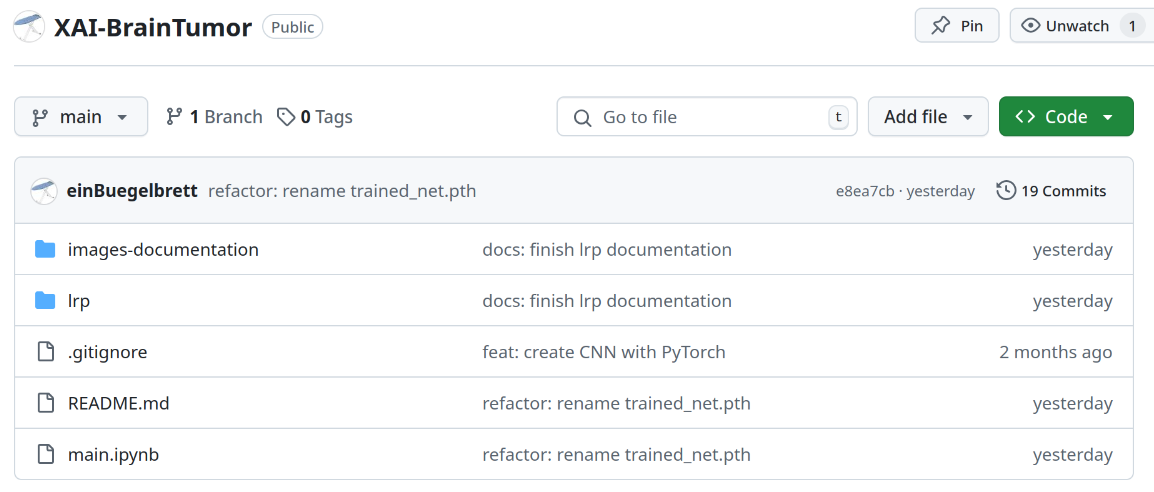
\includegraphics[width=\linewidth]{github}
		\end{frame}
		
		\begin{frame}[t]{Projekt - CNN} \vspace{10pt}
			\centering
			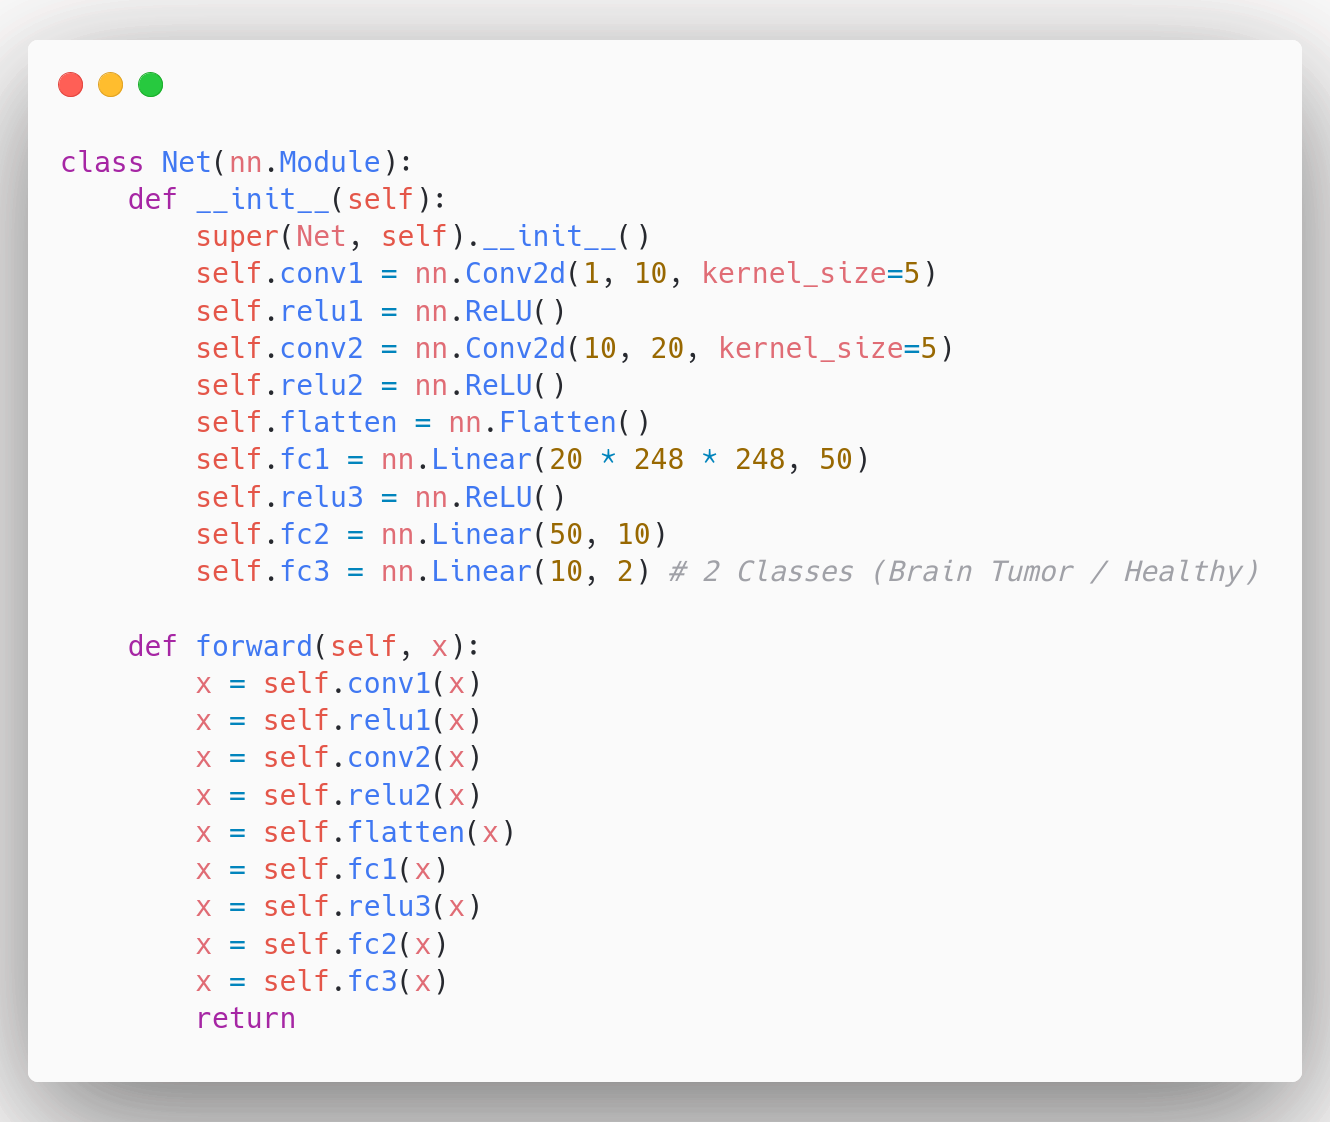
\includegraphics[width=\linewidth, height=0.75\textheight, keepaspectratio]{net}
		\end{frame}
		
		\begin{frame}[t]{Projekt - Konfusionsmatrix} \vspace{10pt}
			\centering
			\includegraphics[width=\linewidth, height=0.75\textheight, keepaspectratio]{confusion\_matrix}
		\end{frame}
		
	\section{LRP}
		\begin{frame}[t]{LRP - Theorie} \vspace{20pt}
			Layer-wise Relevance Propagation (LRP):
			\begin{itemize}
				\item Relevanz von jeden Neuron in ein Neuronales Netz
				\item Foward pass (Vorhersage)
				\item Output wird Schicht für Schicht rückwärts propagiert (Spezielle LRP Regeln)
				\item Heatmap mit dem Beitrag der einzelnen Input-Features (Pixel) zur Vorhersage
			\end{itemize}
		\end{frame}
		
		\begin{frame}[t]{LRP - Theorie - Bild} \vspace*{\fill}
			Hier noch einmal als Bild:
			\begin{center}
				\includegraphics[width=0.3\linewidth]{formula\_1}
			\end{center}
			\includegraphics[width=\linewidth]{lrp\_procedure}
		\end{frame}
		
		\begin{frame}[t]{LRP - Dateistruktur} \vspace{20pt}		
			\begin{figure}[h]
				\centering
				\scalebox{0.9}{
					\begin{forest}
						for tree={
							font=\ttfamily,
							grow'=0,
							child anchor=west,
							parent anchor=south,
							anchor=west,
							calign=first,
							edge path={
								\noexpand\path [draw, \forestoption{edge}]
								(!u.south west) +(7.5pt,0) |- node[fill,inner sep=1.25pt] {} (.child anchor)\forestoption{edge label};
							},
							before typesetting nodes={
								if n=1
								{insert before={[,phantom]}}
								{}
							},
							fit=band,
							before computing xy={l=15pt},
						},
						s=0.1
						[...
						[lrp
						[\_\_init\_\_.py]
						[lrp.py]
						[lrp\_filter.py]
						[lrp\_layers.py]
						]
						[...]
						]
					\end{forest}
				}
			\end{figure} 
		\end{frame}
		
		\begin{frame}[t]{LRP - Implementierung}
			 \vspace*{\fill}
			 \centering
			\includegraphics[width=\linewidth, height=0.75\textheight, keepaspectratio]{lrp\_code}
		\end{frame}
		
	\section{Beobachtungen}
	
		\begin{frame}[t]{Beobachtungen - Gehirntumor}
			\begin{columns}[T, onlytextwidth]
				\column{0.20\textwidth}
				\vspace{90pt}
				Gehirntumor erkannt
				
				\column{0.80\textwidth}
				\vspace{20pt}
				\includegraphics[width=\linewidth]{brain\_tumor\_3}
			\end{columns}
		\end{frame}

		\begin{frame}[t]{Beobachtungen - Gehirntumor}
			\begin{columns}[T, onlytextwidth]
				\column{0.20\textwidth}
				\vspace{90pt}
				Gehirntumor erkannt (mit Hirnhaut)
				
				\column{0.80\textwidth}
				\vspace{20pt}
				\includegraphics[width=\linewidth]{brain\_tumor\_2}
			\end{columns}
		\end{frame}
	
		\begin{frame}[t]{Beobachtungen - Gehirntumor}			
			\begin{columns}[T, onlytextwidth]
				\column{0.20\textwidth}
				\vspace{60pt}
					Auge/Tumor? \\
					$\rightarrow$ wenige Datensätze mit Augen
				
				\column{0.80\textwidth}
				\vspace{20pt}
					\includegraphics[width=\linewidth]{eyes\_brain\_tumor}
			\end{columns}
		\end{frame}
		
		\begin{frame}[t]{Beobachtungen - Gesund} 
			\begin{columns}[T, onlytextwidth]
				\column{0.20\textwidth}
				\vspace{50pt}
					Bild mit wenigen Details\\
					$\rightarrow$  Hirnhaut, ohne Auffälligkeiten 
				
				\column{0.80\textwidth}
					\vspace{20pt}
					\includegraphics[width=\linewidth]{reconize\_h\_1}
			\end{columns}
		\end{frame}
		
		\begin{frame}[t]{Beobachtungen - Gesund} 
			\begin{columns}[T, onlytextwidth]
				\column{0.20\textwidth}
					\vspace{60pt}
					Bild mit vielen Details\\
					$\rightarrow$ Gehirnform entscheidend
				\column{0.80\textwidth}
					\vspace{20pt}
					\includegraphics[width=\linewidth]{reconize\_h\_2}
			\end{columns}
		\end{frame}
		
	\section{Fazit}
		\begin{frame}[t]{Fazit - LRP Vorteile/Nachteile} \vspace{20pt}
			\begin{columns}[T, onlytextwidth]
				\column{0.45\textwidth}
				Vorteile:
				\begin{itemize}
					\item Relevante Merkmale als Heatmap
					\item Die Gesamtrelevanz auf allen Ebenen bleibt erhalten
				\end{itemize}
				
				\column{0.45\textwidth}
				Nachteile
				\begin{itemize}
					\item Ähnliche Merkmale können unabhängig von der untersuchten Klasse hervorgehoben werden
					\item Irrelevante Informationen können hervorgehoben werden
				\end{itemize}
			\end{columns}
		\end{frame}
		
		\begin{frame}[t]{Fazit - Reflexion} \vspace*{\fill}
			\begin{columns}[T, onlytextwidth]
				\column{0.45\textwidth}
				Erfolge:
				\begin{itemize}
					\item Klare Heatmaps
					\item ''Mathe'' umsetzen
				\end{itemize}
				
				\column{0.45\textwidth}
				Schwierigkeiten:
				\begin{itemize}
					\item Datensatz
					\item Optimierung CNN: zuerst 70\% dann 95\%
				\end{itemize}
			\end{columns}
		\end{frame}
		
		\begin{frame}[t]{Fazit - Literaturverzeichnis} \vspace{20pt}
			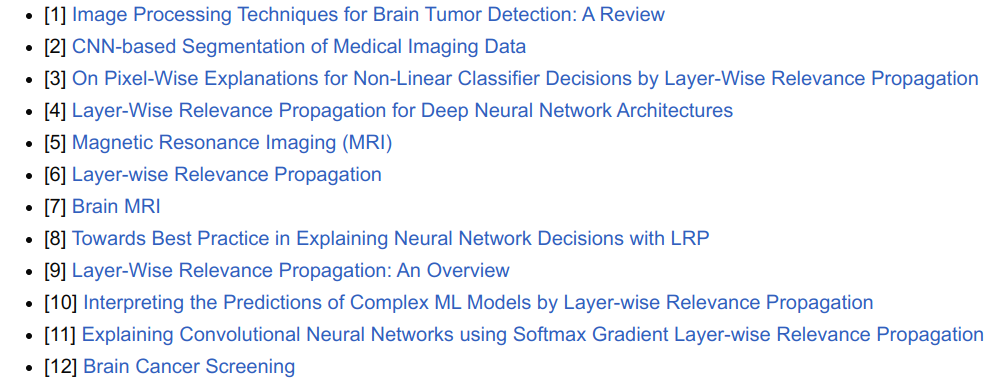
\includegraphics[width=\linewidth]{references}
		\end{frame}
	
	\finalpage{\inserttitlegraphic}
\end{document}